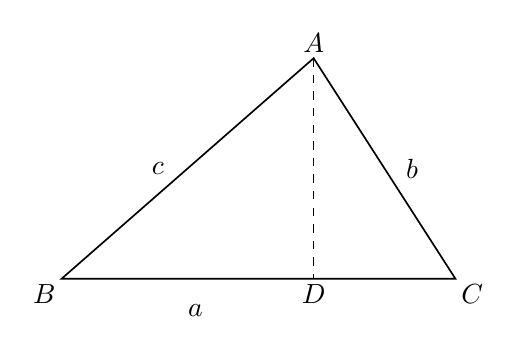
\begin{tikzpicture}[x=1cm,y=1cm,font=\normalsize,
 geometry edge/.style={solid,line width=.6pt},
 geometry mark/.style={solid,line width=.6pt},
 geometry label/.style={font=\normalsize,inner sep=2pt}]
\coordinate (A) at (3.2,2.8);
\coordinate (B) at (0,0);
\coordinate (C) at (5,0);
\coordinate (D) at (3.2,0);
\draw[geometry edge] (A)--(B)--(C)--cycle;
\draw[geometry edge,dashed] (A)--(D);
\node[font=\normalsize,inner sep=2pt] at (1.7,-0.4) {$a$};
\node[font=\normalsize,inner sep=2pt] at (4.45,1.4) {$b$};
\node[font=\normalsize,inner sep=2pt] at (1.22,1.4) {$c$};
\node[geometry label,above] at (A) {$A$};
\node[geometry label,below left] at (B) {$B$};
\node[geometry label,below right] at (C) {$C$};
\node[geometry label,below] at (D) {$D$};
\end{tikzpicture}
